\chapter{Calorimetry and dual-readout}
Calorimetry is an important detection principle in particle physics.
Originally developed with astrophysical purpose for cosmic-ray studies, this method refers to the detection of particles and the measurement of their properties, using blocks of instrumented material.
It was developed and perfected for accelerator-based particle physics experimentation primarily in order to measure the energy of particles. 
In these blocks, particles are fully absorbed and their energy transformed into a measurable quantity.\\
The incident particle interact with the detector (through electromagnetic or strong processes) producing a shower of secondary particles with progressively degraded energy.
The energy deposited by the charged particles of the shower in the active material of the calorimeter, which can be detected in the form of charge or light, is used to measure the energy of the incident particle.
Typical processes suitable to detect this energy are: ionization of the medium, scintillation light and the Cherenkov light produced by relativistic particles.\\

Calorimeters can be divided into two categories depending on the type of shower they are optimized to detect: electromagnetic calorimeters, used mainly to measure electrons and photons through their electromagnetic interactions (e.g.
bremsstrahlung, pair production), and hadronic calorimeters, used to measure mainly hadrons through their strong and electromagnetic interactions.\\
Another classification can be made according to their construction technique defining sampling calorimeters and homogeneous calorimeters.\\
Homogeneous calorimeters are built of one type of material that performs both the main tasks: degrade the energy of the incident particles and provide the detectable signal.\\
Sampling calorimeters, instead, consist of alternating layers of an absorber, a dense material used to perform energy degradation, and an active medium that generate the signal.\\

%Calorimeters are attractive in high-energy particle physic field for various reasons:
%\begin{itemize}
%		\item In most cases the calorimeter energy resolution improves with energy as $1/\sqrt{E}$, where $E$ is the energy of the incident particle. Therefore calorimeters are very well suited to high-energy physics experiments.
%		\item Calorimeters are sensitive to all types of particles, charged and neutral (e.g., neutrons). Also neutrinos and their energy can be indirectly detected can even provide indirect detection of neutrinos and their energy through the measurement of the event missing energy.
%		\item They are versatile detectors. They can be used to determine the shower position and direction, to perform particle identification, to measure the arrival time of the particle, or even to provide fast signals useful in trigger purpose.
%		\item They are space and therefore cost effective. Because the shower length increases only logarithmically with energy, the detector thickness needs to increase only logarithmically with the energy of the particles.
%\end{itemize}

This chapter describes the physics behind both the electromagnetic and hadronic shower developments, provides a basic description of the energy response of these detectors and introduces the particular technique of the dual-readout, a modern concept of calorimeter that has the quality of overcome the non-compensating problem measuring both electromagnetic and hadronic showers through two different type of signals simultaneously (Cherenkov and scintillation light).\\

A more comprehensive descriptions of the topic can be found in the references \cite{Wigmans_book} and \cite{Gianotti_article}.

\section{Physics of shower development}
A particle interact and lose part or whole of its energy traversing matter. During this process the medium get excited and heated up, is excited in this process, or heated up. From this feature the term calorimetry, literally meaning "heat measurement", was introduced.\\
The groundwork for the calorimetry is the interaction processes between particle and matter. They are the manifestation of the electromagnetic, the strong and, more rarely, the weak forces and they strongly depend on the energy and the nature of the incident particle, in addition to medium features.\\
The term particle shower refers to the production of a group of particles generated by the interaction of a primary particle with the matter. The processes and the consequent shower effects are the keys to deeply understand this topic.\\

\subsection{Electromagnetic showers} \label{subsec:em_shower}
Despite the complex mechanisms of particle-matter interaction, electromagnetic showers are produced via a small number of well understood QED processes. Charged particles (electrons and positrons) lose energy by ionization and by radiation, instead neutral ones (photons) are characterized by photoelectric effect, Compton scattering and pair production.

\subsubsection*{Electrons and positrons}
The charged particles, in their path through the medium ionize it under the condition of having an energy at least sufficient to release the atomic electrons from the Coulomb fields generated by the atomic nuclei (few of $eV$).
The amount of energy released (in unit of path) by these particle is predictable through the semi-empirical Bethe-Block formula restricted to electrons (and positrons):
\begin{equation}
    -\frac{dE}{dx} = 2\pi N_a r_e^2 m_e c^2 \rho \frac{Z}{A}\frac{1}{\beta^2}\left[ \ln{\frac{\tau^2(\tau + 2)}{2(I/m_ec^2)^2}} -F(\tau) -\delta -2\frac{C}{Z}\right]
\end{equation}
this formula will not be described in details (see \cite{Leo}). The ionization process is the greatest source of energy loss for particles with small energy.\\
The other energy loss process known as \textit{bremsstrahlung} is the dominant source of energy loss by electrons and positrons at energies above $100\ MeV$. Relativistic electrons and positrons radiate photons as a result of the interaction between Coulomb and the atomic electric fields. The energy spectrum of these photons falls off as $1/E$ ranging till the primary particle energy, but in general most of the photons carry a small part of it.
The process produces (usually small) changes in electron (or positron) direction. This is called Coulomb or multiple scattering.\\
At a fixed energy the relative importance of ionization and radiation losses depends on the medium and in particular on the electron density of the medium in which the shower develops. This density is in first approximation proportional to the (average) $Z$ of the medium.
The critical energy, i.e. the energy value at which both processes have equal impact, is roughly inversely proportional to the $Z$ value of the material:
\begin{equation}
    \varepsilon_c = \frac{160\ MeV}{Z + 1.24}.
\end{equation}
An example of energy loss in copper by electron is sketched in figure \ref{fig:Cu_rad_ion}, where the ionization and radiation contribution are separated.

\begin{figure}
	\centering
	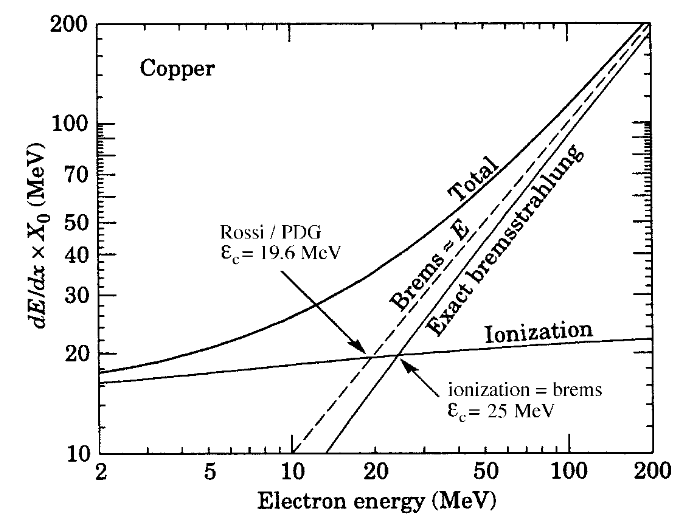
\includegraphics[width=0.8\textwidth]{IMG/Cap2/Cu_rad_ion}
	\caption{Energy losses through ionization and bremsstrahlung by  electrons in copper. From [PDG 98].}
	\label{fig:Cu_rad_ion}
\end{figure}

\subsubsection*{Photons}
The other particles that produce electromagnetic showers are photons. The interaction between photons and matter is mainly affected by three different processes: the photoelectric effect, Compton scattering and electron–positron pair production.\\

The photoelectric effect is the process that most likely occurs at low energies. It is characterized by an atom absorbing the photon and emitting an electron. Eventually the atom, left in an excited state, emits an Auger electrons or X-rays returning to the ground state. The photoelectric cross section strongly depends on the available number of  electrons,  and  thus  on  the $Z$ value  of  the  absorber  material. In particular it scales with $Z^n$, with the power $n$ between 4 and 5. Meanwhile the photoelectric cross section rapidly decrease with greater energies, varying as $E^{-3}$. In this way the process rapidly loses its impact as the energy increases. Quantitatively, in uranium ($Z=92$) the cross section for photoelectric effect is dominant for energies below $700\ keV$, meanwhile for iron  ($Z=26$) decreases his importance from $100\ keV$.\\

The Compton process is a scattering process where an impinging  photon interact with an atomic electron transferring enough momentum and energy to the struck electron to escape from the atomic Coulomb field. The dynamic is illustrated in Figure \ref{fig:scatt_kin}. Kinematic variables such as energy transfer and scattering angles can be easily obtained applying the laws of energy and momentum conservation. 

\begin{figure}
	\centering
	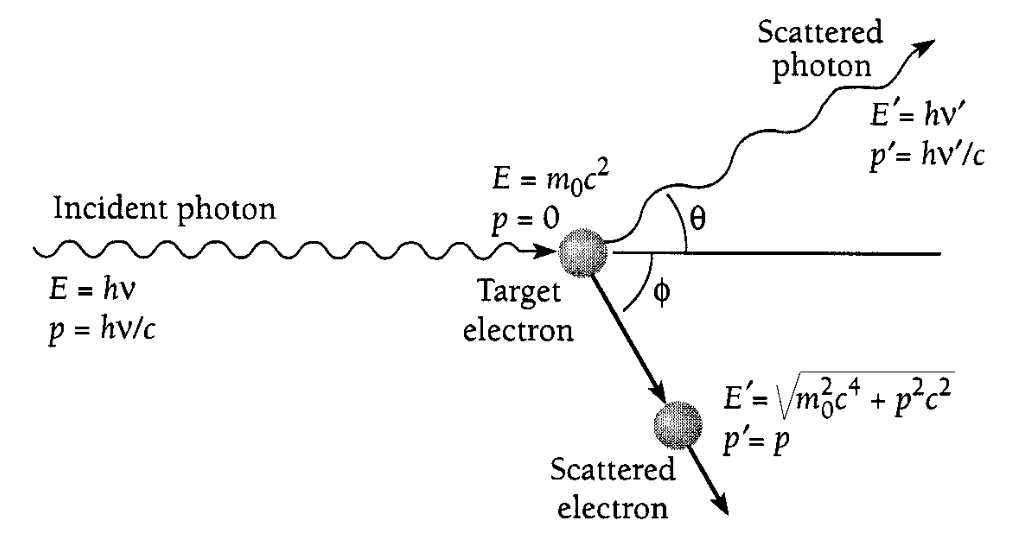
\includegraphics[width=0.8\textwidth]{IMG/Cap2/scatt_kin.png}
	\caption{Compton scattering process. Image from \cite{Leo}.}
	\label{fig:scatt_kin}
\end{figure}

The photon is absorbed and thus disappears in the photoelectric effect, but it only plays a role at low $\gamma$ energies. Photons in the $MeV$ energy range are absorbed only after a sequence of Compton scattering processes, in which the photon energy is reduced step by step in each collision until it is low enough to permit the photoelectric occurrence. In each step, the amount of loss energy is:
\begin{equation}
    T = E_{\gamma}\frac{\xi(1 - \cos{\theta})}{1 + \xi(1 - \cos{\theta})}
\end{equation}
where $\xi = E_{\gamma}/m_ec^2$.
The cross section linked to the Compton scattering is much less dependent on the $Z$ value than the photoelectric one. It is almost proportional to the number of target electrons in the nuclei. Also in this process the cross section decreases with increasing photon energy, but only with the first power of $E$. Therefore Compton scattering has more impact than photoelectric absorption above a certain threshold energy. This  threshold varies from $20\ keV$ for carbon ($Z=6$) to $700\ keV$ for uranium ($Z=92$).\\

The pair production process, differently from the previous ones, has a binding threshold under which the effect can not occur. This threshold is the twice of the electron rest mass ($1.022\ GeV$). If the photon has a higher energy then it can produce an electron-positron pair that can continue the path in the medium producing bremsstrahlung radiation as well as ionization.
The electron can be eventually absorbed by an ion, while the positron annihilates with an electron producing two new photons, each with an energy of $511\ keV$.

The cross section for pair production does not decreases with the photon energy as in photoelectric effect and in Compton scattering, instead it rises with the energy reaching an asymptotic value at higher then $1\ GeV$. For this reason, at high energies, pair production is the most likely process to occur.
Meanwhile the dependence from the medium goes, in first approximation, as $Z^2$.\\

Comparing the cross section of the three processes and its dependence with respect to the photon energy it is clear that the photoelectric effect dominates at lower energies, meanwhile at the intermediate values the Compton scattering gives the greatest contribute, at the end at higher energies almost every photon loses its energy through pair production. An example of these contributions is shown in figure \ref{fig:ph_cross_E}.\\
Knowing the dependence of the cross sections with respect to the $Z$ of the material, ranges of energies where each process dominates can be found and parametrized with the $Z$ value. A representation is sketched in figure \ref{fig:ph_cross_Z}.\\ 

%\begin{figure}
%	\centering
%	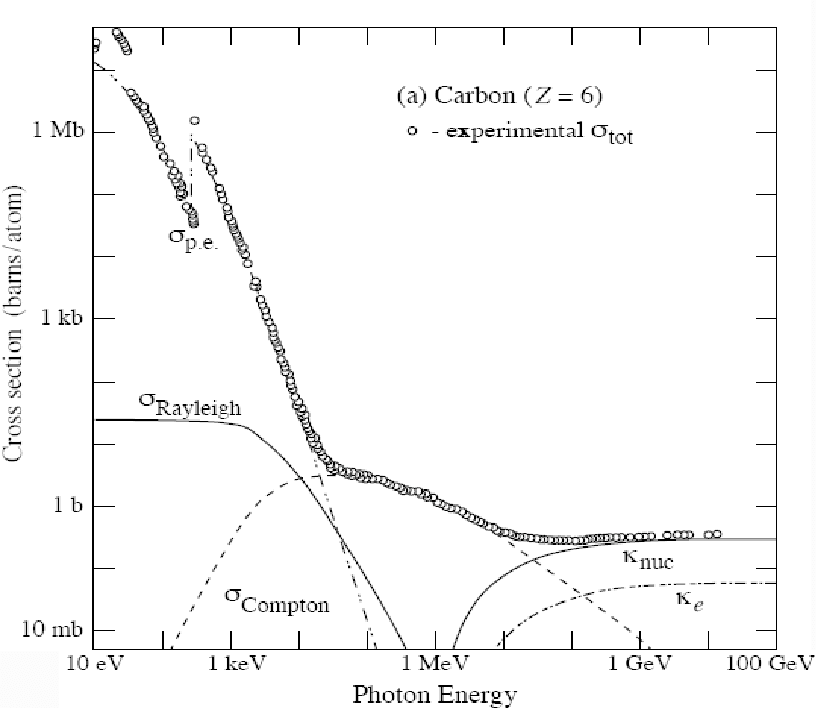
\includegraphics[width=0.7\textwidth]{IMG/Cap2/ph_cross_E.png}
%	\caption{Compton scattering process. Image from \cite{Leo}.}
%	\label{fig:ph_cross_E}
%\end{figure}
%\begin{figure}
%	\centering
%	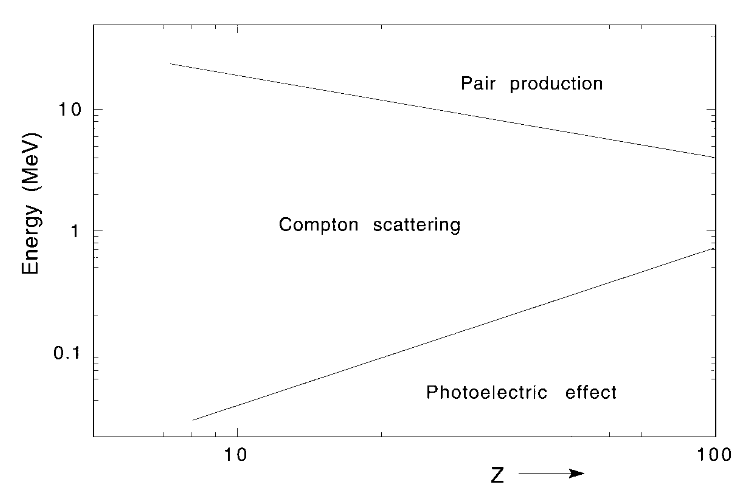
\includegraphics[width=0.7\textwidth]{IMG/Cap2/ph_cross_Z.png}
%	\caption{Compton scattering process. Image from \cite{Leo}.}
%	\label{fig:ph_cross_Z}
%\end{figure}

\begin{figure}
	\centering
	\subfloat[][Total cross section of photon in Carbon. Different processes contribution are also separated. \label{fig:ph_cross_E}]{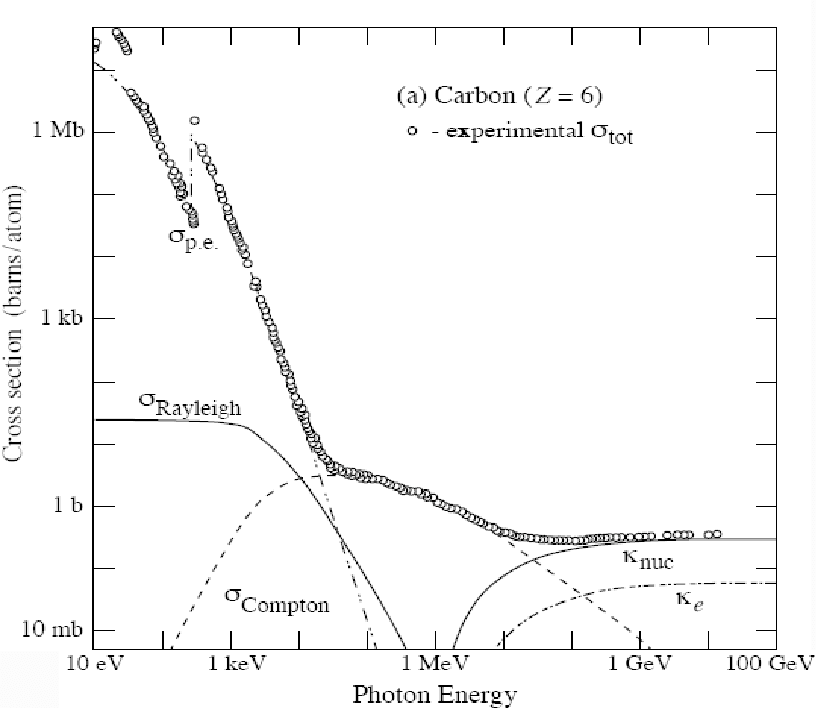
\includegraphics[height=.18\textheight]{IMG/Cap2/ph_cross_E.png}} \quad
	\subfloat[][Energy ranges where different processes dominate with respect to the medium $Z$ value.\label{fig:ph_cross_Z}]{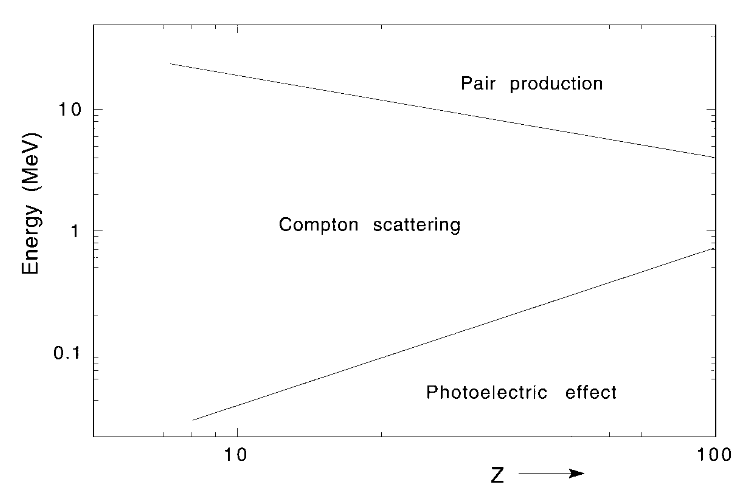
\includegraphics[height=.18\textheight]{IMG/Cap2/ph_cross_Z.png}}
	\caption{Images from \cite{Leo}.}
	%\label{fig:sigma_su_e}
\end{figure}

\subsubsection*{Shower principle}
Minimal showers may also develop at vary low energy of primary particle. Starting for example from a photon of few $MeV$, it can eventually produce a electron-positron pair in the calorimeter. The  charged  particles lose their energy in the matter through ionization. When the  positron loses all the kinetic energy, it annihilates with an electron producing two $511\ keV\ \gamma$s. These photons are absorbed through the photoelectric effect after a sequence of Compton scattering. During the process, the energy of the primary particle is released to the material by charged particle in ionization processes

At energies of $1\ GeV$ and higher, electrons and photons initiate em showers in the materials in which they penetrate. Electrons lose their energy predominantly by radiation, the most energetic photons pro-duced in this process convert intoe+e−pairs, which radiate moreγs,etc.The number of shower particlesproduced in this particle multiplication process reaches a maximum (theshower maximum) at a certaindepth inside the absorber, and gradually decreases beyond that depth (Figure 2a). The depth of the showermaximum increases (logarithmically) with the energy of the incoming electron. 



\subsection{Hadronic showers} \label{subsec:had_shower}
aaa

\section{Energy response of calorimeters}
aaa

\subsection{Homogeneous calorimeters}
aaa

\subsection{Sampling calorimeters}
aaa

\subsection{Compensation}
aaa

\section{Dual-readout calorimetry}
aaa

\subsection{Working principles}
aaa

\subsection{Experiments}